
\begin{figure}[]
  \begin{center}
    %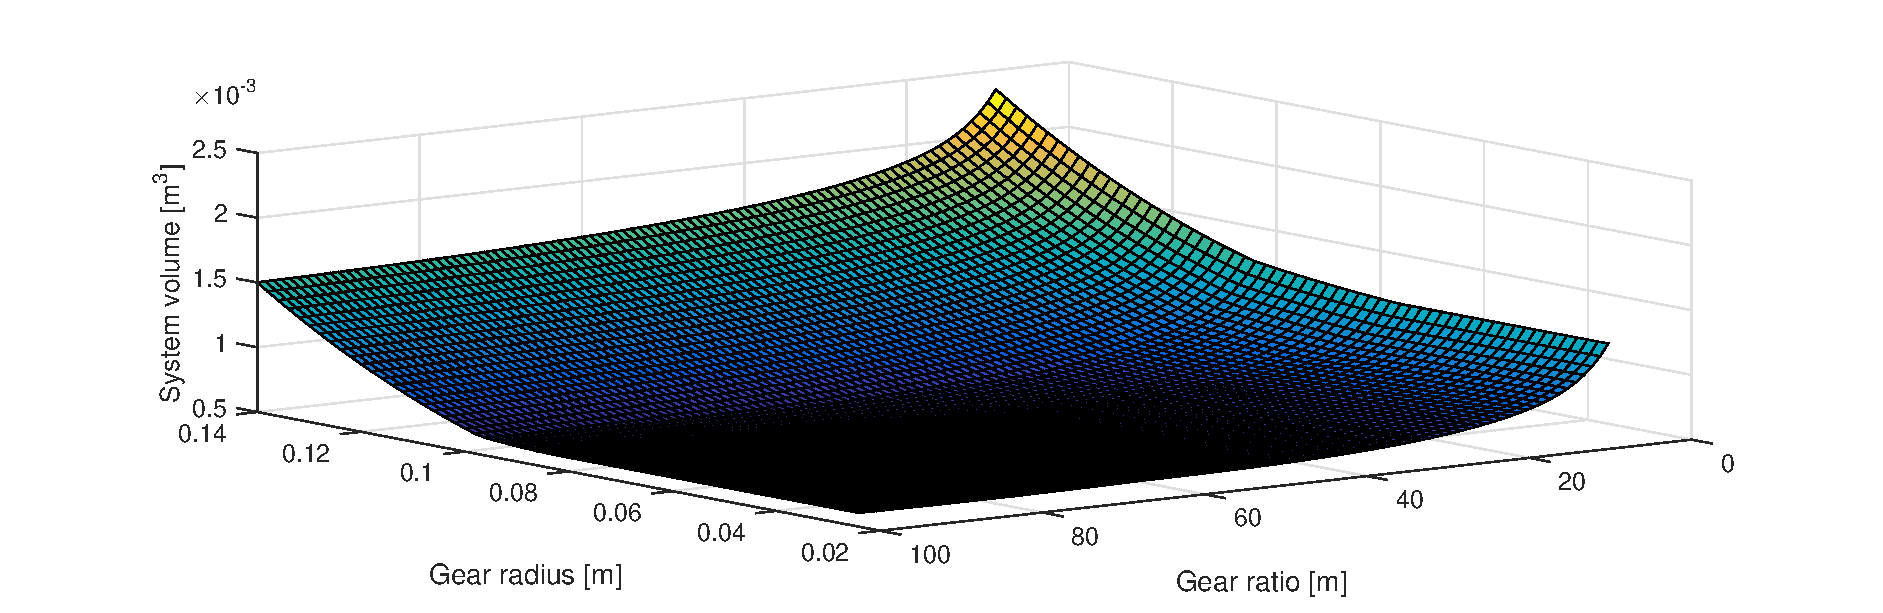
\includegraphics[width=\linewidth]{Plots/3Dplot_convex_static_mediumQ.eps}
    \missingfigure[figwidth=\linewidth]{Testing a long text string}
  \end{center}
  \caption{Mechatronics servo system consisting of a motor and planetary gear which serves as the design case.}
  \label{fig:CaseSystem}
\end{figure}

The physical system studied in our case is a mechatronic servo system consisting of a motor, a shaft and two planetary gear stages; as shown in figure \ref{fig:CaseSystem}. Both the static and dynamic models for different components have been previously developed by Roos and Malmquist. The load inertia, $J_{\text{load}}$, for the presented design case is as 1.1$kg/m^2$ and the chosen load profile can be viewed in Figure \ref{???}. This scenario is equivalent to the one presented by Malmquist in order to perform a fair comparison. The dimensioning factor introduced in the dynamic model is according to Malmquist$'$s method applied to all the valid results from the static model, while in our case, the dimensioning factor is only calculated for the optimum from the static models.

%From figure ??? [[[[we can see]]] that the peak torque is $T_{peak}=191.4 N/m$ and the root mean square (RMS) value of torque $T_{RMS} = 49.39 N/m$. Similarly, the optimization objective is still the system volume.    

\subsection*{Models}
This section will focus on how to convert the excising mathematical models of the components in our design case to geometrical forms which can be analysed in the CVX software. 
\subsubsection*{Motor}
The motor model was derived by Roos\cite{roos2007} based on the constraint that the rated torque should be no less than the expected RMS torque according to
\begin{equation} \label{eq:cs1}
T_{\text{m,rated}} \geq \tilde{T}_{\text{m}}.
\end{equation}
Furthermore, Roos derived the rated torque of the motor considering mechanical, magnetic and thermal effects as
\begin{equation} \label{eq:cs2}
T_{\text{m,rated}}=C_{\text{m}}l_{\text{m}} r_{\text{m}}^{2.5}
\end{equation}
where $C_{\text{m}}$ is a constant for a specific motor type and cooling condition, $l_{\text{m}}$ is the motor length and $r_{\text{m}}$ the radius of the stator. The RMS torque required from the motor is derived by propagating the load torque $T_{\text{l}}$ through the planetary gear with gear ratio $n$
\begin{equation} \label{eq:cs3}
\tilde{T}_{\text{m}}=\sqrt{\frac{1}{\tau}\int_0^\tau ((C_{\text{mj}}l_{\text{m}} r_{\text{m}}^{4}+J_{\text{m}})\ddot{\varphi}_{\text{m}}+\frac{T_{\text{l}}}{n})^2  \mathrm{d} t}
\end{equation}
where $C_{\text{mj}}$ is constant for a specific motor type and derived from a reference motor of the same type, $J_{\text{m}}$ is the rotor inertia ${\varphi}_{\text{m}}$ is the angular position of the output shaft.
Rewriting the equation \ref{eq:cs1} by combining equation \ref{eq:cs2} and \ref{eq:cs3} results in
\begin{equation} \label{eq:cs4}
C_{\text{m}}l_{\text{m}} r_{\text{m}}^{2.5}\geq \sqrt{\frac{1}{\tau}\int_0^\tau ((C_{\text{mj}}l_{\text{m}} r_{\text{m}}^{4}+J_{\text{m}})\ddot{\varphi}_{\text{m}}+\frac{T_{\text{l}}}{n})^2  \mathrm{d} t}.
\end{equation}
Hence, the geometric form of this constraint can then be stated as
\begin{equation} \label{eq:cs5}
\frac{n_{\text{j}}^2 n^2 C_{\text{mj}}^2 T_{\text{rms}}^2 r_{\text{m}}^3}{J_{\text{load}}^2} + \frac{2 n_{\text{j}} C_{\text{mj}} T_{\text{rms}}^2}{J_{\text{load}} r_{\text{m}} l_{\text{m}}} + \frac{T_{\text{rms}}^2}{n^2 l_{\text{m}}^2 r_{\text{m}}^5}\leq C_{\text{m}}^2
\end{equation}
where $n_{\text{j}}$ is defined as $\frac{C_{\text{mj}}l_{\text{m}} r_{\text{m}}^{4}+J_{\text{m}}}{C_{\text{mj}}l_{\text{m}} r_{\text{m}}^{4}}$ and approximated as 10/9. 

A complementary constraint for the motor model is form factor constraint
\begin{equation} \label{eq:cs6}
0.5 \leq \frac{l_{\text{m}}}{r_{\text{m}}} \leq 5
\end{equation}

The dynamic model of the motor is derived as
\begin{equation} \label{eq:cs7}
K_{\text{t}}i= \frac{T_{\text{l}}}{n} + J_{\text{m}}\ddot{{\varphi}}_{\text{m}}
\end{equation}
where $K_{\text{t}}$ is the constant and $i$ is the electric current.


\subsubsection*{Planetary gear}
A planetary gear consisting of a sun gear, three planet gears and a ring gear is used in the servo system //Nescessary?//instead of a spur gear since the volume of the planetary gear is less than a spur gear when transmitting the same torque////. The main constraints on the planetary gear are bending stress in the root of a gear teeth and Hertzian pressure at the teeth contact surfaces. However, if the number of the sun gear teeth is small and/or the the gears are made from ductile steel, the dominant constraint would be the Herzian pressure. Every teeth surface needs to fulfil 
\begin{equation} \label{eq:cs8}
r_{\text{g}}^2b \geq Z_{\text{H}}^2 Z_{\text{M}}^2 Z_{\epsilon} K_{\text{H} \alpha} K_{\text{H} \beta} \frac{T_{\text{l}}(n-1)^2}{6(n-2)\sigma_{\text{H,max}}^2}.
\end{equation}
according to Roos. Applying the standard parameters defined in Roos$'$ work, equation \ref{eq:cs8} can be simplified as
\begin{equation} \label{eq:cs9}
r_{\text{g}}^2b \geq 4\cdot10^{10} \cdot C_{\text{gr}}^2\frac{T_{\text{l}}(n-1)^2}{(n-2)\sigma_{\text{H,max}}^2}
\end{equation}
where $C_{\text{gr}}$ is the ratio of the outer gear radius and the gear$'$s pitch radius; $\sigma_{\text{H,max}}$ is the maximum allowed flank pressure given by
\begin{equation} \label{eq:cs10}
\sigma_{\text{H,max}}=\frac{\sigma_{\text{H,lim}}}{SF}
\end{equation}
where $\sigma_{\text{H,lim}}$ is the maximum allowed Herzian pressure for the particular gear material and $SF$ is the safe factor.

The geometric form to replace the equation \ref{eq:cs9} is expressed as
\begin{equation} \label{eq:cs11}
\frac{(n-1)^2}{(n-2)} \approx n+\sum_{i=0}^{\infty} \frac{1}{n}\times(\frac{2}{n})^i = \frac{(n-1)^2-(\frac{2}{n})^i}{n-2}
\end{equation}

The equation \ref{eq:cs11} holds when the term $(\frac{2}{n})^i$ is sufficiently small, which can be satisfied by $n \gg 2$ and the number of the sum terms $i$ is sufficiently large. 

\subsubsection*{Shaft}
The static model for the shaft is derived from the classic solid mechanics. The following equations are from Collins[????]
\begin{equation} \label{eq:cs12}
r_{\text{s}} = \sqrt[3]{\frac{2\tilde{T}_{\text{s,out}}}{\tau_{\text{s,max}} \pi}}
\end{equation}
\begin{equation} \label{eq:cs13}
J_{\text{s}} = \frac{\pi r_{\text{s}}^4}{2}
\end{equation}
\begin{equation} \label{eq:cs14}
G = \frac{E}{2(1+\nu)}
\end{equation}
\begin{equation} \label{eq:cs15}
k = \frac{GJ_{\text{s}}}{l}
\end{equation}
where $r_{\text{s}}$ is the shaft radium, $\tilde{T}_{\text{s,out}}$ is the maximum transferred torque, $\tau_{\text{s,max}}$ is the maximum permissible shear stress, $J_{\text{s}}$ is the shaft polar moment of inertia, $G$ is the shear modulus, $E$ is Young$'$s modulus, $\nu$ is Poisson$'$s ratio, $l$ is the length and $k$ is the stiffness of the shaft.
 
The shaft dynamic behavior is approximated as a spring-damper model. The equations are derived as
\begin{equation} \label{eq:cs16}
\frac{1}{2}J_{\text{s}}\ddot{\varphi}_{\text{s,in}} = T_{\text{s,in}}-k(\varphi_{\text{s,in}}-\varphi_{\text{s,out}})-d(\dot{\varphi}_{\text{s,in}}-\dot{\varphi}_{\text{s,out}})
\end{equation}
\begin{equation} \label{eq:cs17}
\frac{1}{2}J_{\text{s}}\ddot{\varphi}_{\text{s,out}} = k(\varphi_{\text{s,in}}-\varphi_{\text{s,out}})+d(\dot{\varphi}_{\text{s,in}}-\dot{\varphi}_{\text{s,out}})-T_{\text{s,out}}.
\end{equation}
\subsubsection*{Load}
Load does not have a static model as a physical component does. However, the dynamic model exists and derived as
\begin{equation} \label{eq:cs18}
J_{\text{l}}\ddot{\varphi}_{\text{l}} = T_{\text{l}}
\end{equation}
where $J_{\text{l}}$ is the load inertia and $T_{\text{l}}$ is the load torque.  
\subsection*{Results Comparision}
After arranging the static constraints of different components to geometric form, the physical system would be optimized for volume from the aspects of both static and dynamic using CVX toolbox. The optimization results as well as computing time would be recorded to be compared with Malmquist$'$ work. 
After running CVX, the values for different design variables as well as computing time are obtained and recorded along with those from GA  in table????? and table ?????
table?                                     
\begin{table}[h]
\caption{Static model results}
\label{sta}
\begin{center}
\begin{tabular}{|c||c||c|}
\hline
Comparison Item & Convex Optimization & Genetic Algorithm\\
\hline
$Three$ & $Four$ & $Four$\\
\hline
$Three$ & $Four$ & $Four$\\
\hline
$Three$ & $Four$ & $Four$\\
\hline
$Three$ & $Four$ & $Four$\\
\hline
$Three$ & $Four$ & $Four$\\
\hline
\end{tabular}
\end{center}
\end{table}

In dynamic model, ISE is calculated by applying the discrete state space method mentioned above to the closed loop transfer function with all the poles chosen at $-150$ beforehand. The expression for ISE is $k$, which only depends on $k$ since $k$ is the only design variable contained in the numerator of the closed loop transfer function. As observed, the expression yields a parabolic curve regarding $\frac{1}{k}$. An explanation could be that ISE increases as $k$ decreases since a softer shaft causes bigger overshoot when $k<k_o$ and ISE increases as $k$ increases since a stiffer shaft causes bigger lag time when $k>k_o$.
It can be seen that convex optimization returns the results with allowed error while the computing time is much shortened compared with genetic algorithm. 
\begin{table}[h]
\caption{Dynamic model results}
\label{dyn}
\begin{center}
\begin{tabular}{|c||c||c|}
\hline
Comparison Item & Convex Optimization & Genetic Algorithm\\
\hline
$Three$ & $Four$ & $Four$\\
\hline
$Three$ & $Four$ & $Four$\\
\hline
$Three$ & $Four$ & $Four$\\
\hline
$Three$ & $Four$ & $Four$\\
\hline
$Three$ & $Four$ & $Four$\\
\hline
\end{tabular}
\end{center}
\end{table}

\begin{figure}[t]
  \begin{center}
    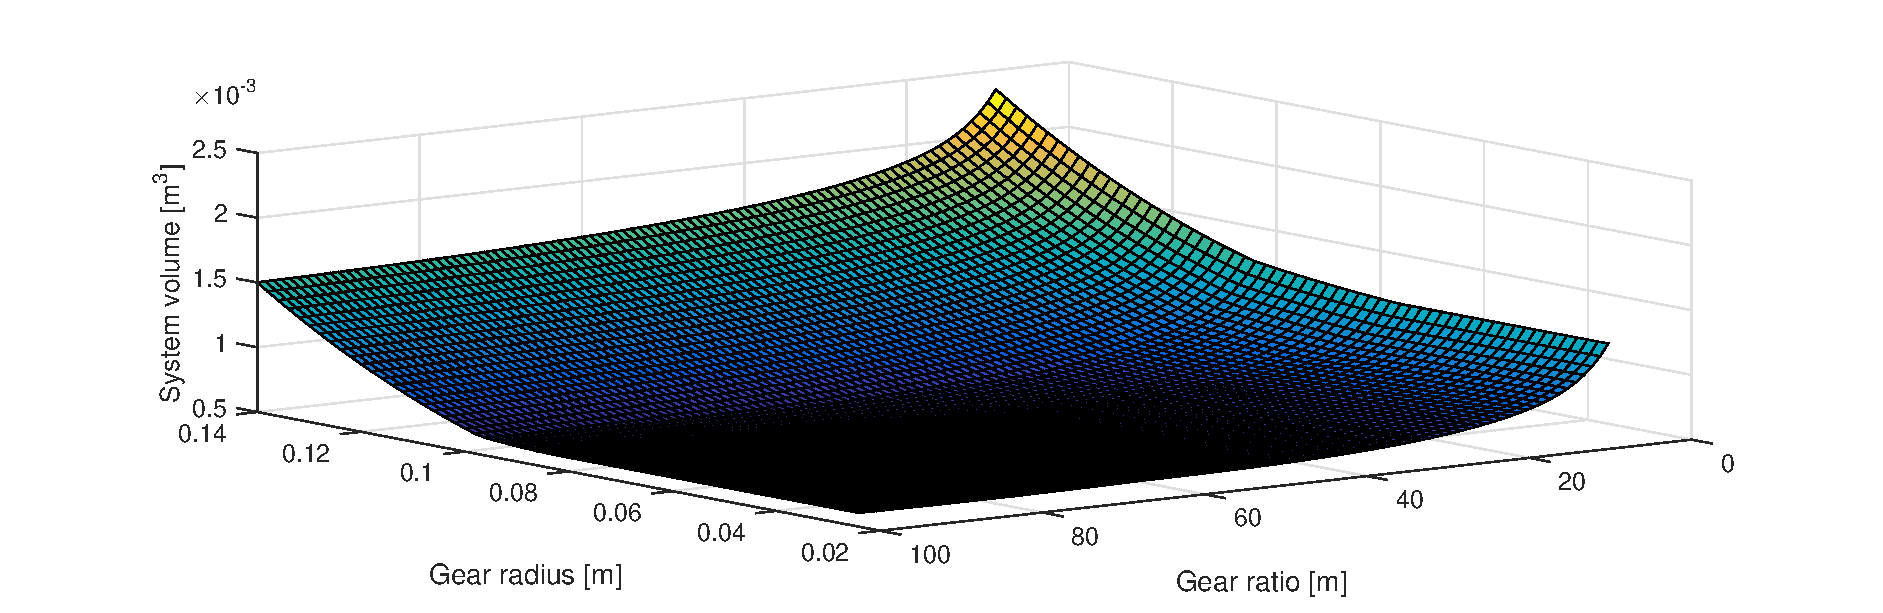
\includegraphics[width=\linewidth]{Plots/3Dplot_convex_static_mediumQ.eps}
  \end{center}
  \caption{Optimal volume for static case with varying gear radius and gear ratio.}
  \label{fig:static3D}
\end{figure}


